\documentclass[11pt]{article}
\usepackage{enumitem}
\usepackage{listings}
\usepackage[listings]{tcolorbox}
\usepackage{tikz}
\usepackage{url}

%\usepackage{algorithm2e}
\usetikzlibrary{arrows,automata,shapes}
\tikzstyle{block} = [rectangle, draw, fill=blue!20, 
    text width=5em, text centered, rounded corners, minimum height=2em]
\tikzstyle{bt} = [rectangle, draw, fill=blue!20, 
    text width=4em, text centered, rounded corners, minimum height=2em]

\lstset{ %
language=Java,
basicstyle=\ttfamily,commentstyle=\scriptsize\itshape,showstringspaces=false,breaklines=true,numbers=left}
\newtcbinputlisting{\codelisting}[3][]{
    extrude left by=1em,
    extrude right by=2em,
    listing file={#3},
    fonttitle=\bfseries,
    listing options={basicstyle=\ttfamily\footnotesize,numbers=left,language=Java,#1},
    listing only,
    hbox,
}
\lstdefinelanguage{JavaScript}{
  keywords={typeof, new, true, false, catch, function, return, null, catch, switch, var, if, in, while, 
do, else, case, break},
  keywordstyle=\color{blue}\bfseries,
  ndkeywords={class, export, boolean, throw, implements, import, this},
  ndkeywordstyle=\color{darkgray}\bfseries,
  identifierstyle=\color{black},
  sensitive=false,
  comment=[l]{//},
  morecomment=[s]{/*}{*/},
  commentstyle=\color{purple}\ttfamily,
  stringstyle=\color{red}\ttfamily,
  morestring=[b]',
  morestring=[b]''
}


\newtheorem{defn}{Definition}
\newtheorem{crit}{Criterion}

\newcommand{\handout}[5]{
  \noindent
  \begin{center}
  \framebox{
    \vbox{
      \hbox to 5.78in { {\bf Software Testing, Quality Assurance and Maintenance } \hfill #2 }
      \vspace{4mm}
      \hbox to 5.78in { {\Large \hfill #5  \hfill} }
      \vspace{2mm}
      \hbox to 5.78in { {\em #3 \hfill #4} }
    }
  }
  \end{center}
  \vspace*{4mm}
}

\newcommand{\lecture}[4]{\handout{#1}{#2}{#3}{#4}{Lecture #1}}
\topmargin 0pt
\advance \topmargin by -\headheight
\advance \topmargin by -\headsep
\textheight 8.9in
\oddsidemargin 0pt
\evensidemargin \oddsidemargin
\marginparwidth 0.5in
\textwidth 6.5in

\parindent 0in
\parskip 1.5ex
%\renewcommand{\baselinestretch}{1.25}

\begin{document}

\lecture{3 --- January 13, 2025}{Winter 2025}{Patrick Lam}{version 1}

We're going to continue talking about testing for now. This week, I
also plan to talk about fuzzing. Then we'll shift gears---we are going to
talk about operational semantics, which is the invisible foundation for the
proofs that you saw in SE 212. Making the semantics visible makes the proofs doable by machine.

\section*{When to stop? Idea 1: Coverage}

So, in the testing space, we write a bunch of tests and hope it's good
enough. For most of us, it's never that fun to write tests. But, you
want to do a good job, so you should write some number of tests. What
is that number?

If you could test your function or program on every single input (and
if you had an oracle to tell you if the output was correct), then that
would clearly be enough. This doesn't work. Even if your program is
not timing-sensitive. There are just too many inputs. That's
exponential growth for you.

Short of that, one metric that people use in industry is the notion of
code coverage. In particular, statement coverage and branch coverage.
There are other notions of coverage, but they are not widely used and
I don't think they actually tell you anything useful.

You could evaluate statement coverage and branch coverage based on
program source code. But that's a bit ambiguous. We use control-flow
graphs instead.

\paragraph{Aside: white-box and black-box testing.} I don't think this
is really a big deal these days, but there is the term \emph{white-box} testing,
which means that you can look at the source code when you write tests,
and \emph{black-box} testing, where you can't.

The fundamental graph for
source code is the \emph{Control-Flow Graph} (CFG), which originates
from compilers.

\begin{itemize}
\item CFG nodes: a node represents zero or more statements;
\item CFG edges: an edge $(s_1, s_2)$ indicates that $s_1$ may
  be followed by $s_2$ in an execution.
\end{itemize}

\paragraph{Example.} Consider the following code.
\begin{lstlisting}
  x = 5;
  for (z = 2; z < 17; z++)
    print(x);
\end{lstlisting}

Recall the steps in compilation:
\begin{itemize}
\item lexing: input = stream of characters, output = stream of tokens (if, while, strings)
\item parsing: input = stream of tokens, output = concrete syntax tree
\item construction of Abstract Syntax Tree (AST): cleans up the concrete syntax tree
\item conversion to Control Flow Graph: input = AST, output = CFG
\item optimizations: input = CFG, output = CFG
\item convert to bytecode/machine code: input = CFG, output = bytecode/machine code
\end{itemize}

The Abstract Syntax Tree corresponding to the example code might look like this:

\begin{center}
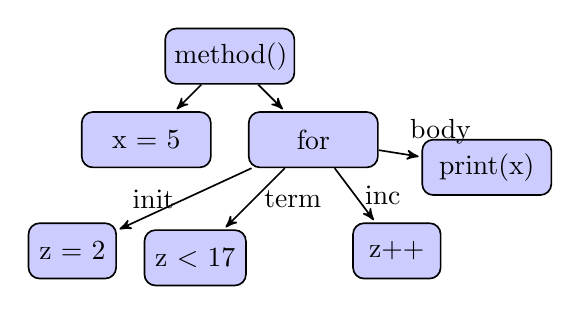
\begin{tikzpicture}[->,>=stealth',shorten >=1pt,auto,node distance=1.5cm,
                    semithick,initial text=]

  \node[bt]           (1) {method()};
  \node[bt]           (2) [below left of=1] {x = 5};
  \node[bt]           (3) [below right of=1] {for};
  \node[bt]           (4) [right of=3,xshift=2em,yshift=-1em] {print(x)};
  \node[bt, text width=2.5em]           (5) [below left of=3,xshift=-2cm,yshift=-1em] {z = 2};
  \node[bt, text width=3em]           (6) [below of=3,xshift=-1.5cm] {z $<$ 17};
  \node[bt, text width=2.5em]           (7) [below right of=3,yshift=-1em] {z++};

  \path (1) edge node {} (2)
  (1) edge node {} (3)
  (3) edge node {body} (4)
  (3) edge node[left] {init} (5)
  (3) edge node[right] {term} (6)
  (3) edge node[right] {inc} (7);
\end{tikzpicture}
\end{center}

\paragraph{From ASTs to CFGs.}

We can convert the Abstract Syntax Tree into the following Control Flow Graph.
\begin{center}
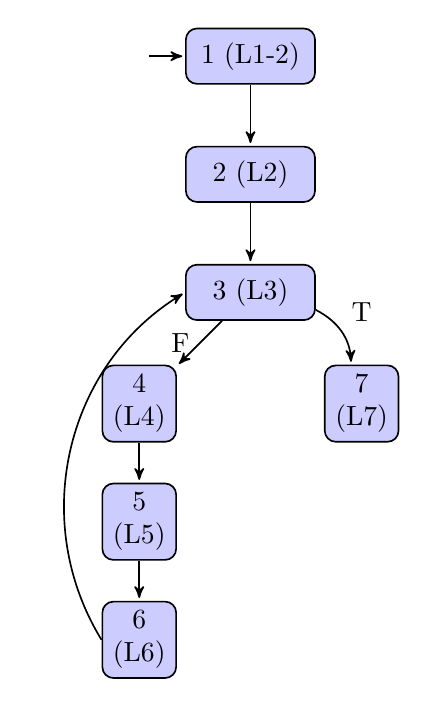
\begin{tikzpicture}[->,>=stealth',shorten >=1pt,auto,node distance=1.5cm,
                    semithick,initial text=]

  \node[initial,bt]   (1)                     {1 (L1-2)};
  \node[bt]           (2) [below of=1]        {2 (L2)};
  \node[bt]           (3) [below of=2] {3 (L3)};
  \node[bt, text width=2em]           (4) [below left of=3,xshift=-1em,yshift=-1em] {4 (L4)};
  \node[bt, text width=2em]           (5) [below of=4,yshift=0em] {5 (L5)};
  \node[bt, text width=2em]           (6) [below of=5,yshift=0em] {6 (L6)};
  \node[bt, text width=2em]           (7) [below right of=3,xshift=1em,yshift=-1em] {7 (L7)};

  \path (1) edge node {} (2)
        (2) edge node {} (3)
        (3) edge node[left] {F} (4)
            edge [bend left] node {T} (7)
        (4) edge node {} (5)
        (5) edge node {} (6)
        (6.west) edge [bend left=45] node {} (3.west);
\end{tikzpicture}
\end{center}

\newpage
\paragraph{From CFG to low-level code.}
And we can convert the CFG into the following low-level code:
\begin{lstlisting}
    x = 5
    z = 2
q0: if (z < 17) goto q1
    z = z + 1
    print (x)
    goto q0
q1: nop
\end{lstlisting}

\paragraph{Basic Blocks.} We can simplify a CFG by grouping together
statements which always execute together (in sequential programs):

\begin{center}
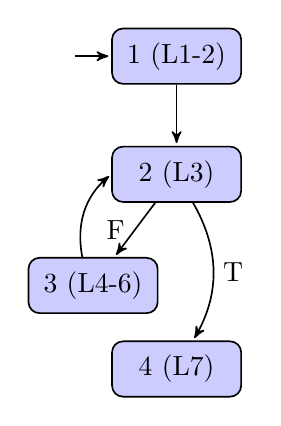
\begin{tikzpicture}[->,>=stealth',shorten >=1pt,auto,node distance=1.5cm,
                    semithick,initial text=]

  \node[initial,bt]   (1)                     {1 (L1-2)};
  \node[bt]           (2) [below of=1] {2 (L3)};
  \node[bt]           (3) [below left of=2,yshift=-1em] {3 (L4-6)};
  \node[bt]           (4) [below right of=3] {4 (L7)};

  \path (1) edge node {} (2)
        (2) edge node[left] {F} (3)
            edge [bend left] node {T} (4)
        (3) edge [bend left] node {} (2.west);
\end{tikzpicture}
\end{center}

We use the following definition:
\begin{defn}
A basic block is a sequence of instructions in the control-flow graph
that has one entry point and one exit point.
\end{defn}
We are usually interested in forming maximal basic blocks.
Note that a basic block may have multiple successors. However, there 
may not be any jumps into the middle of a basic block (which is
why statement {\tt l0} has its own basic block.)

\paragraph{Constructing CFGs.} This is a mechanical process which I don't want to talk about much.

{\bf if statements:} One can put the conditions
(and hence uses) on the control-flow edges, rather than in the 
{\tt if} node. I prefer putting the condition in the node.

\begin{tabular}{ll|ll}
\begin{minipage}{.15\textwidth}
\scriptsize \begin{lstlisting}
if (z < 17)
  print (x);
else
  print (y);
\end{lstlisting}
\end{minipage} &
\begin{minipage}{.3\textwidth}
\begin{center}
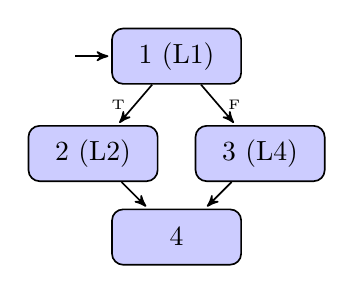
\begin{tikzpicture}[->,>=stealth',shorten >=1pt,auto,node distance=1.5cm,
                    semithick,initial text=]

  \node[initial,bt]   (1)                     {1 (L1)};
  \node[bt]           (2) [below left of=1,yshift=-0.5em] {2 (L2)};
  \node[bt]           (3) [below right of=1,yshift=-0.5em] {3 (L4)};
  \node[bt]           (4) [below left of=3] {4};

  \path (1) edge node[left] {\tiny T} (2)
        (1) edge node[right] {\tiny F} (3)
        (2) edge node {} (4)
        (3) edge node {} (4);
\end{tikzpicture}
\end{center}
\end{minipage}&
\begin{minipage}{.25\textwidth}
\begin{center}
\begin{tikzpicture}[->,>=stealth',shorten >=1pt,auto,node distance=1.5cm,
                    semithick,initial text=]

  \node[initial,bt]   (1)                     {1 (L1)};
  \node[bt]           (2) [below left of=1,yshift=-0.5em] {2 (L2)};
  \node[bt]           (4) [below left of=3] {3};

  \path (1) edge node[left] {\tiny T} (2)
        (1) edge node[right] {\tiny F} (4)
        (2) edge node {} (4);
\end{tikzpicture}
\end{center}
\end{minipage}
& \scriptsize \begin{minipage}{.2\textwidth}
\begin{lstlisting}
if (z < 17)
  print(x);
\end{lstlisting}
\end{minipage}
\end{tabular}

Short-circuit {\tt if} evaluation is more complicated; I recommend working it out yourself.

{\bf case / switch statements:} 

\begin{tabular}{ll}
\begin{minipage}{.45\textwidth}
\begin{lstlisting}
switch (n) {
  case `I': ...; break;
  case `J': ...; // fall thru
  case `K': ...; break;
}
// ...
\end{lstlisting}
\end{minipage} &
\begin{minipage}{.4\textwidth}
\begin{center}
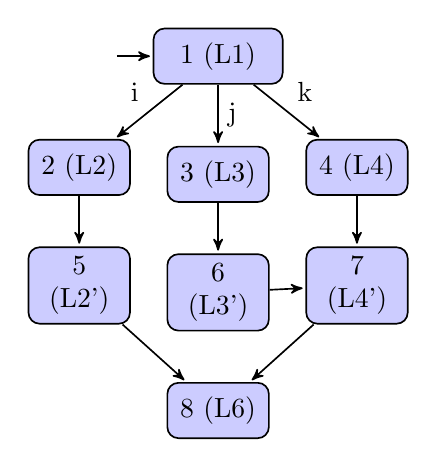
\begin{tikzpicture}[->,>=stealth',shorten >=1pt,auto,node distance=1.5cm,
                    semithick,initial text=]

  \node[initial,bt]   (1)                     {1 (L1)};
  \node[bt, text width=3em]           (2) [below left of=1,xshift=-2em,yshift=-1em]  {2 (L2)};
  \node[bt, text width=3em]           (3) [below of=1]   {3 (L3)};
  \node[bt, text width=3em]           (4) [below right of=1,xshift=2em,yshift=-1em]   {4 (L4)};
  \node[bt, text width=3em]           (5) [below of=2]  {5 (L2')};
  \node[bt, text width=3em]           (6) [below of=3]  {6 (L3')};
  \node[bt, text width=3em]           (7) [below of=4]  {7 (L4')};
  \node[bt, text width=3em]           (8) [below of=6]  {8 (L6)};

  \path 
  (1) edge node[left,yshift=0.7em] {i} (2)
  (1) edge node {j} (3)
  (1) edge node {k} (4)
  (2) edge node {} (5)
  (3) edge node {} (6)
  (4) edge node {} (7)
  (6) edge node {} (7)
  (5) edge node {} (8)
  (7) edge node {} (8);
\end{tikzpicture}
\end{center}
\end{minipage}
\end{tabular}

{\bf while statements:}

\begin{tabular}{ll}
\begin{minipage}{.2\textwidth}
\begin{lstlisting}
x = 0; y = 20;
while (x < y) {
  x ++; y --;
}
\end{lstlisting}
\end{minipage} &
\begin{minipage}{.4\textwidth}
\begin{center}
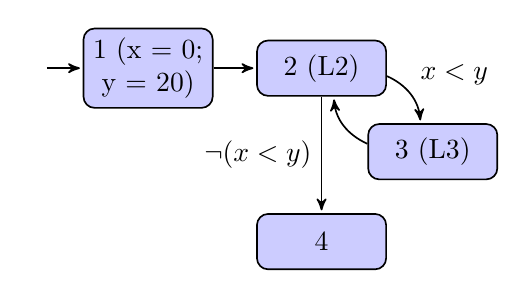
\begin{tikzpicture}[->,>=stealth',shorten >=1pt,auto,node distance=1.5cm,
                    semithick,initial text=]

  \node[initial,bt]   (1)                     {1 (x = 0; y = 20)};
  \node[bt]           (2) [right of=1,xshift=2em]        {2 (L2)};
  \node[bt]           (3) [below right of=2,xshift=1em]  {3 (L3)};
  \node[bt]           (4) [below of=2,yshift=-2em]   {4};

  \path (1) edge node {} (2)
  (2) edge [bend left] node {$x < y$} (3)
  (3) edge [bend left] node {} (2)
  (2) edge node[left] {$\neg (x < y)$} (4);
\end{tikzpicture}
\end{center}
\end{minipage}
\end{tabular}

Note that arbitrarily complicated structures may occur inside
the loop body.

    {\bf for statements:} 

\begin{tabular}{ll}
\small
  \begin{minipage}{.5\textwidth}
\begin{lstlisting}
for (int i = 0; i < 57; i++) {
  if (i % 3 == 0) {
    print (i);
  }
}
\end{lstlisting}
\end{minipage} & \begin{minipage}{.4\textwidth}
  (an exercise for the reader; \\ 
we saw one earlier!)
\end{minipage}
\end{tabular}

This example uses Java's enhanced for loops, which iterates over all of the elements
in the {\tt widgetList}:

\begin{lstlisting}[basicstyle=\scriptsize \ttfamily]
for (Widget w : widgetList) {
  decorate(w);
}
\end{lstlisting}

Either the simplified one or the more useful one on the right are OK:

\begin{tabular}{ll}
\begin{minipage}{.4\textwidth}
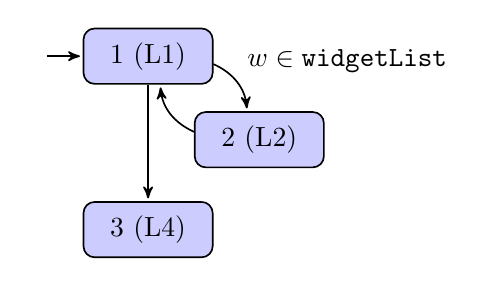
\begin{tikzpicture}[->,>=stealth',shorten >=1pt,auto,node distance=1.5cm,
                    semithick,initial text=]

  \node[initial,bt]   (1)                     {1 (L1)};
  \node[bt]           (3) [below right of=1,xshift=1em]  {2 (L2)};
  \node[bt]           (4) [below of=1,yshift=-2em]   {3 (L4)};

  \path 
  (1) edge [bend left] node {$w \in \mbox{\tt widgetList}$} (3)
  (3) edge [bend left] node {} (1)
  (1) edge node[left] {} (4);
\end{tikzpicture}
\end{minipage} &
\begin{minipage}{.5\textwidth}
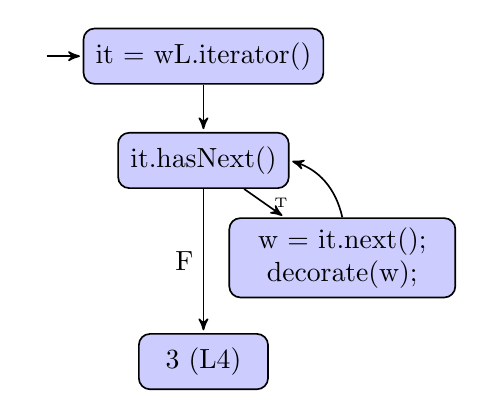
\begin{tikzpicture}[->,>=stealth',shorten >=1pt,auto,node distance=1.5cm,
                    semithick,initial text=]

  \node[initial,bt,text width=8em]   (1)                     {it = wL.iterator()};
  \node[bt,text width=5.5em]            (2) [below of=1,yshift=.5em] {it.hasNext()};
  \node[bt,text width=7.5em]           (3) [below right of=2,xshift=2em,yshift=-.5em]  {w = it.next(); decorate(w);};
  \node[bt]           (4) [below of=2,yshift=-3em]   {3 (L4)};

  \path (1) edge node {} (2)
        (2) edge node[right] {\tiny T} (3)
        (3.north) edge [bend right] node {} (2.east)
        (2) edge node[left] {F} (4);
%  (1) edge [bend left] node {$w \in \mbox{\tt widgetList}$} (3)
%  (3) edge [bend left] node {} (1)
%  (1) edge node[left] {} (4);
\end{tikzpicture}
\end{minipage}
\end{tabular}


\subsection*{Statement \& Branch Coverage}

I used to give a more formal definition, but it boils down to this.
You have a test suite and a program. For this purpose, the program is
expressed in terms of a set of CFGs (one per method).

Instrument the program to count whether each statement (control-flow
node) is executed or not.  Also instrument it to count whether each
branch (control-flow edge) is taken or not.

\emph{Statement coverage} is the fraction of statements (nodes) that are
executed by the test suite. \emph{Branch coverage} is the fraction of branches (edges)
that are executed.

[Should give an example]


\subsection*{Infeasible Test Requirements; How Much Coverage, Anyway?}

% [was L14]
For toy programs, we can reach 100\% statement and branch coverage.
For real programs, this is still theoretically possible, but becomes
impractical. 

We'll wrap up our unit on defining test suites by exploring the question
``How much is enough?'' We'll discuss coverage first and then mutation testing
as ways of answering this question.

First, we can look at actual test suites and see how much coverage they achieve.
I collected this data a few years ago, measured with the EclEmma tool.

\begin{center}
  \includegraphics[height=2in]{L03/coverage.png}
\end{center}

We can see that the coverage varies between 20\% and 95\% on actual
open-source projects. I investigated further and found that while Weka has low
test coverage, it instead uses scientific peer review for QA: its features
come from published articles. Common practice in industry is that about 80\%
coverage (doesn't matter which kind) is good enough.

There is essentially no quantitative analysis of input space coverage;
for most purposes, input spaces are essentially infinite.

Let's look at a more specific case study, JUnit. The rest of this lecture is
based on a blog post by Arie van Deursen:

\begin{center}
  \url{https://avandeursen.com/2012/12/21/line-coverage-lessons-from-junit/}
\end{center}

Although you might think of JUnit as something that just magically exists in the world,
it is a software artifact too. JUnit is written by developers who obviously really care
about testing. Let's see what they do.

Here's the Cobertura report for JUnit:

\begin{center}
  \includegraphics[height=2in]{L03/cobertura-junit.png}
\end{center}

\paragraph{Stats.} Overall instruction (statement) coverage for JUnit 4.11 is about 85\%; there are
13,000 lines of code and 15,000 lines ot test code. (It's not that
unusual for there to be more tests than code.) This is consistent with
the industry average.

\paragraph{Deprecated code?} Sometimes library authors decide that some functionality
was not a good idea after all. In that case they might \emph{deprecate} some methods or
classes, signalling that these APIs will disappear in the future.

In JUnit, deprecated and older code has lower coverage levels. Its 13 deprecated
classes have only 65\% instruction coverage. Ignoring deprecated code, JUnit achieves
93\% instruction coverage. Furthermore, newer code in
package {\tt org.junit.*} has 90\% instruction coverage, while older code in
{\tt junit.*} has 70\% instruction coverage.

(Why is this? Perhaps the coverage decreased over time for the deprecated code, since
no one is really maintaining it anymore, and failing test cases just get removed.)

\paragraph{Untested class.} The blog post points out one class that was completely
untested, which is unusual for JUnit. It turns out that the code came with tests,
but that the tests never got run because they were never added to any test suites.
Furthermore, these tests also failed, perhaps because no one had ever tried them.
The continuous integration infrastructure did not detect this change. (More on CI
later.)

\paragraph{What else?} Arie van Deursen characterizes the remaining 6\% as
``the usual suspects''. In JUnit's case, there was no method with more than
2 to 3 uncovered lines. Here's what he found.

\noindent
\emph{Too simple to test.} Sometimes it doesn't make sense to test a method, because
it's not really doing anything. For instance:
\begin{lstlisting}[language=Java]
  public static void assumeFalse(boolean b) {
    assumeTrue(!b);
  }
\end{lstlisting}
or just getters or {\tt toString()} methods (which can still be wrong).

The empty method is also too simple to test; one might write such a method to allow
it to be overridden in subclasses:
\begin{lstlisting}[language=Java]
  /**
  * Override to set up your specific external resource.
  *
  * @throws if setup fails (which will disable {@code after}
  */
  protected void before() throws Throwable {
    // do nothing
  }
\end{lstlisting}

\noindent \emph{Dead by design.} Sometimes a method really should never be called,
for instance a constructor on a class that should never be instantiated:
\begin{lstlisting}[language=Java]
  /**
  * Protect constructor since it is a static only class
  */
  protected Assert() { }
\end{lstlisting}

A related case is code that should never be executed:
\begin{lstlisting}[language=Java]
  catch (InitializationError e) {
    throw new RuntimeException(
    "Bug in saff's brain: " +
    "Suite constructor, called as above, should always complete");
  }
\end{lstlisting}
Similarly, switch statements may have unreachable default cases. Or other unreachable code.
Sometimes the code is just highly unlikely to happen:
\begin{lstlisting}[language=Java]
  try {
    ...
  } catch (InitializationError e) {
    return new ErrorReportingRunner(null, e); // uncovered
  }
\end{lstlisting}

\paragraph*{Conclusions.} We explored empirically the instruction coverage of JUnit,
which is written by people who really care about testing. Don't forget
that coverage doesn't actually guarantee, by itself, that your code is
well-exercised; what is in the tests matters too. For non-deprecated
code, they achieved 93\% instruction coverage, and so it really is
possible to have no more than 2-3 untested lines of code per
method. It's probably OK to have lower coverage for deprecated
code. Beware when you are adding a class and check that you are also
testing it.



\section*{Fuzzing}

Consider the following JavaScript code\footnote{\url{http://webkit.sed.hu/blog/20130710/fuzzinator-mutation-and-generation-based-browser-fuzzer}}.
\begin{lstlisting}[language=JavaScript]
function test() {
    var f = function g() {
        if (this != 10) f();
    };
    var a = f();
}
test();
\end{lstlisting}
Turns out that it can crash WebKit (\url{https://bugs.webkit.org/show_bug.cgi?id=116853}).
Plus, it was automatically generated by the Fuzzinator tool, based on a grammar for JavaScript.

Fuzzing is the modern-day implementation of the input space based
grammar testing that we talked about in last time. While the
fundamental concepts were in the earlier lecture, we will see how
those concepts actually work in practice.  Fuzzing effectively finds
software bugs, especially security-based bugs (caused, for instance,
by a lack of sufficient input validation.)

\paragraph{Origin Story.} It starts with line noise.
In 1988, Prof. Barton Miller was using a 1200-baud dialup modem to
communicate with a UNIX system on a dark and stormy night.  He found
that the random characters inserted by the noisy line would cause his
UNIX utilities to crash. He then challenged graduate students in his
Advanced Operating Systems class to write a fuzzer---a program which
would generate (unstructured ASCII) random inputs for other programs.
The result: the students observed that 25\%-33\% of UNIX utilties
crashed on random inputs\footnote{\url{http://pages.cs.wisc.edu/~bart/fuzz/Foreword1.html}}.
% footnote: fuzzing book foreword

(That was not the earliest known example of fuzz testing. Apple
implemented ``The Monkey'' in 1983\footnote{\url{http://www.folklore.org/StoryView.py?story=Monkey_Lives.txt}}
to generate random events for
MacPaint and MacWrite. It found lots of bugs. The limiting factor was
that eventually the monkey would hit the Quit command.  The solution
was to introduce a system flag, ``MonkeyLives'', and have MacPaint and
MacWrite ignore the quit command if MonkeyLives was true.)
% footnote: folklore.org

\paragraph{How Fuzzing Works.} 
Two kinds of fuzzing: \emph{mutation-based} and
\emph{generation-based}. Mutation-based testing starts with
existing test cases and randomly modifies them to explore new behaviours.
Generation-based testing starts with a grammar and generates
inputs that match the grammar.

One detail that I didn't mention last time was the bug detection
part.  Back then, I just talked about generating interesting
inputs. In fuzzing, you feed these inputs to the program and find
crashes, or assertion failures, or you run the program under a dynamic
analysis tool such as Valgrind and observe runtime errors.

\paragraph{The Simplest Thing That Could Possibly Work.}
Consider generation-based testing for HTML5.  The simplest grammar---actually a regular
expression---that could possibly
work\footnote{\url{http://trevorjim.com/a-grammar-for-html5/}} is {\tt
  .*}, where {\tt .} is ``any character'' and {\tt *} means ``0 or
more''. Indeed, that grammar found the following WebKit assertion failure:
\url{https://bugs.webkit.org/show_bug.cgi?id=132179}.

The process is as described previously. Take the regular expression
and generate random strings from it.  Feed them to the browser and see
what happens. Find an assertion failure/crash.

\paragraph{More sophisticated fuzzing.} Let's say that we're trying to
generate C programs. One could propose the following hierarchy of inputs\footnote{\url{http://www.cs.dartmouth.edu/~mckeeman/references/DifferentialTestingForSoftware.pdf}}:
\begin{enumerate}
\item sequence of ASCII characters;
\item sequence of words, separators, and white space (gets past the lexer);
\item syntactically correct C program (gets past the parser);
\item type-correct C program (gets past the type checker);
\item statically conforming C program (starts to exercise optimizations);
\item dynamically conforming C program;
\item model conforming C program.
\end{enumerate}
Each of these levels contains a subset of the inputs from
previous levels. However, as the level increases, we are more likely
to find interesting bugs that reveal functionality specific
to the system (rather than simply input validation issues).

While the example is specific to C, the concept applies to all
generational fuzzing tools. Of course, the system under test
shouldn't ever crash on random ASCII characters. But it's hard
to find the really interesting cases without incorporating knowledge
about correct syntax for inputs (or, as in the Apple case, excluding
the ``quit'' command). Increasing the level should also increase
code coverage.

John Regehr discusses this issue at greater
length\footnote{\url{blog.regehr.org/archives/1039}} and concludes
that generational fuzzing tools should operate at all levels.

\paragraph{Mutation-based fuzzing.}
In mutation-based fuzzing, you develop a tool that randomly modifies existing
inputs. You could do this totally randomly by flipping bytes in the input,
or you could parse the input and then change some of the nonterminals.
If you flip bytes, you also need to update any applicable
checksums if you want to see anything interesting (similar to
level 3 above).

Here's a description of a mutation-based fuzzing workflow by the author of Fuzzinator.
{\small
\begin{quote}
  More than a year ago, when I started fuzzing, I was mostly focusing on mutation-based fuzzer technologies since they were easy to build and pretty effective. Having a nice error-prone test suite (e.g. LayoutTests) was the warrant for fresh new bugs. At least for a while. As expected, the test generator based on the knowledge extracted from a finite set of test cases reached the edge of its possibilities after some time and didn't generate essentially new test cases anymore. At this point, a fuzzer girl can reload her gun with new input test sets and will probably find new bugs. This works a few times but she will soon find herself in a loop testing the common code paths and running into the same bugs again and again.\footnote{\url{http://webkit.sed.hu/blog/20141023/fuzzinator-reloaded}}
\end{quote}
}
\paragraph{Fuzzing Summary.} Fuzzing is a useful technique for finding
interesting test cases. It works best at interfaces between components.
Advantages: it runs automatically and really works. Disadvantages: without
significant work, it won't find sophisticated domain-specific issues.

\section*{Related: Chaos Monkey}
Instead of thinking about bogus inputs, consider instead what happens
in a distributed system when some instances (components) randomly fail
(because of bogus inputs, or for other reasons). Ideally, the system
would smoothly continue, perhaps with some graceful degradation until
the instance can come back online. Since failures are inevitable, it's
best that they occur when engineers are around to diagnose them and
prevent unintended consequences of failures.

Netflix has implemented this in the form of the Chaos
Monkey\footnote{\url{http://techblog.netflix.com/2012/07/chaos-monkey-released-into-wild.html}}
and its relatives. The Chaos Monkey operates at instance level, while
Chaos Gorilla disables an Availability Zone, and Chaos Kong knocks out
an entire Amazon region. These tools, and others, form the Netflix
Simian
Army\footnote{\url{http://techblog.netflix.com/2011/07/netflix-simian-army.html}}.
%https://github.com/Netflix/SimianArmy/tree/master/assets

Jeff Atwood (co-founder of StackOverflow) writes about experiences with a Chaos Monkey-like system\footnote{\url{http://blog.codinghorror.com/working-with-the-chaos-monkey/}}. Why inflict such a system on yourself? ``Sometimes you don't get a choice; the Chaos Monkey chooses you.'' In his words, software engineering benefits of the Chaos Monkey included:

\begin{itemize}
\item    ``Where we had one server performing an essential function, we switched to two.''
\item    ``If we didn't have a sensible fallback for something, we created one.''
\item    ``We removed dependencies all over the place, paring down to the absolute minimum we required to run.''
\item     ``We implemented workarounds to stay running at all times, even when services we previously considered essential were suddenly no longer available.''
\end{itemize}


% TODO: modify and add content from the fuzzing book
% https://www.fuzzingbook.org/html/Fuzzer.html


\end{document}
